\chapter{Learning Problems}
\chapterauthor{Samuel Ireson}

\begin{chout}
	We now aim to combine the concepts which we have thus far encountered, and construct a formal definition for a learning problem. We will begin by defining the necessary inputs, and the desired outputs, before working towards the fundamental definition of PAC learnability, which will allow us to have some notion of the possibility of learning a certain problem.
\end{chout}

\section{Introduction}
We begin the chapter by laying out an example which we will reference and build around throughout.

Suppose that you are a loaner, aiming to determine if an arbitrary loanee will or will not default on the loan you give them. We phrase the problem deliberately in this manner, to emphasize the simplistic scenario in which we are working -- the value of the loan is predetermined, and the goal is to provide a binary classification of loanees.

What information will be useful in this task? How will we determine if our solution is adequate? How will be provide a useful notation to describe the problem?

\section{A formal learning model \basic}
\subsection{Learning input}
The learner of a statistical learning problem has access to the following,
\begin{itemize}
	\item Domain set: an arbitrary set which we typically label by $ \mathcal{X} $. This set is nothing more than the objects to which we aim to assign labels. In the example outlined in the previous section, this set $ \mathcal{X} $ is the set of potential loanees.
	\item Label set: A set which we typically label by $ \mathcal{Y} $. This is the set of possible labels, e.g., $ \{ \text{default} , \text{no default} \} $. Of course, it is more common to denote the possible labels simply by integers, and in our binary classification example, we will take $ \mathcal{Y}=\{ \pm1 \} $.
	\item Training data: a finite sequence of pairs $ ( x_{i}, y_{i} )\in \mathcal{X}\times \mathcal{Y} $, i.e., a sequence of labelled objects. In our case, this will be a sequence of past loaners together with information relating to their repayment. We will tend to denote the training data by $ \mathcal{S} = ( ( x_{1}, y_{1} ), ..., ( x_{m}, y_{m} ) ) $, where $ m $ is the size of the training data.
\end{itemize}

\begin{figure}[!htb]
	\centering

	\includegraphics{learning-input/figure.pdf}
	\caption{The training set $ \mathcal{S} $ is the collection of points in $ \mathcal{X} $ for which we have labels. The function $ f $ is the true labelling function.}

\end{figure}


\begin{remark}
	It is important to note that the training data is described as a sequence rather than a set. This is a rather nuanced point, and not one which we will dedicate much thought to. The reason for such pedanticity is that there exist learning algorithms which are dependent on the order of the training points, and there is no necessity for $ \mathcal{S} $ to be duplicate free.

	It is however still common to refer to $ \mathcal{S} $ as the training set.
\end{remark}

\subsection{Learning output}
\begin{itemize}
	\item Prediction rule: the only output from a statistical learning problem is a function $ h: \mathcal{X} \to \mathcal{Y} $. We also refer to the function as a hypothesis, and is a rule which the learner can use to label new elements of the domain space.

	      If we are considering an algorithm $ \mathcal{A} $, then we will denote by $ \mathcal{A}( \mathcal{S} ) $ or $ h_{\mathcal{S}} $ the output hypothesis of the algorithm.
\end{itemize}

\subsection{A data generating model}
It is important to consider how exactly the training data is generated, as this is integral to how we consider the learning to occur. We assume that there is some probability distribution $ \mathcal{D} $ over $ \mathcal{X} $ which, importantly, the learner does not know about. For the time being, we also make the assumption that there is some `correct' labelling function $ f: \mathcal{X} \to \mathcal{Y}: x_{i} \mapsto y_{i} $, which maps the object $ x_{i} $ to it's correct label in every case. Explicitly,
\begin{align*}
	f ( x_{i} ) = y_{i} \quad \forall i.
\end{align*}

In every learning scenario, it is exactly this function $ f $ which the learner aims to obtain. In our example, we can suppose that we have past data, $ \mathcal{S} $ which provides a source of truth in the way that each of the training examples is an individual of whom we \textit{know} the loaning outcome.


\subsection{Measure of success}
The final element of our formal learning model is the means to quantify the success of our learning, or more strictly our hypothesis, $ h $. In our classification problem, the error of the hypothesis $ h $ is defined to be the probability that for a given data point $ x \in \mathcal{X} $, the predicted classification is not the same as the `correct' classification. Notatively,
\begin{align*}
	L_{\mathcal{D}, f}( h ) := \mathbb{P}_{x \sim \mathcal{D}}\left[ h ( x ) \neq f ( x ) \right]
\end{align*}

\begin{remark}
	The notation of $ L_{\mathcal{D}, f} $ is well chosen since it makes clear the dependence of the error of the classifier on the underlying distribution $ \mathcal{D} $ and correct classification function $ f $, although if the context is clear we will omit this for brevity.

	It is also common to refer to the probability $ L_{\mathcal{D}, f}( h ) $ as the `risk', and we will often refer to it as such.
\end{remark}

\section{Empirical Risk Minimisation \intermediate}
We now have a good idea about the inputs, outputs and measures of success of a formal learning problem. The natural next step is to explore the strategy by which we can solve such problems.

It maybe initially seems obvious that we would like to minimise the risk, explicitly reducing the probability of incorrect classification, implicitly bringing our hypothesis output $ h $ closer to the true classifier $ f $. Although this is the right idea, we are the learner is limited by their knowledge of the problem. In particular, the learning knows nothing of the distribution $ \mathcal{D} $, nothing of the true classifier $ f $, and hence nothing of the risk $ L_{\mathcal{D}, f} $. As a result, we must construct a different quantity which we would like to minimise.

\begin{definition}[Empirical risk]
	Given a training sequence $ \mathcal{S} = ( ( x_{1}, y_{1} ), ..., ( x_{m}, y_{m} ) ) $, the \defined{empirical risk} with respect to $ \mathcal{S} $ is defined and denoted by,
	\begin{align*}
		L_{\mathcal{S}}( h ) := \frac{|\left\{ i \in \{ 1,...,m \}: h ( x_{i} ) \neq f ( x_{i} ) \right\}|}{m}
	\end{align*}
\end{definition}

This definition is basic in spite of it's verbosity. The numerator is expressing the process of counting misclassifications on the training set, and we are dividing by the size of the training set to ensure that $ L_{\mathcal{S}} $ is bounded between $ 0 $ and $ 1 $.

The empirical risk is a good quantity to consider in learning problems since it is related to the training data available to us, i.e., ``the snapshot of the world available to the learner''\cite{schwartz}. So, our strategy of learning comes down to minimising the empirical risk -- finding a hypothesis $ h $, which agrees well with $ f $ on the training set. Learning by this strategy is called \defined{empirical risk minimisation}, referred to by $ \mathrm{ERM} $.

\subsection{Overfitting}
We now explore a pitfall into which many learning algorithms fall, and one which we will illustrate using the framework so far developed in this chapter, working again with the example of loaning.

\begin{example}
	In order to illustrate overfitting in the $ \mathrm{ERM} $ paradigm, we suppose that the underlying distribution $ \mathcal{D} $ on loan applicants $ \mathcal{X} $ is uniform, that is, the correct classification of the feature space is half-half between default ($ 1 $) and non-default ($ -1 $).

	It may seem initially that the process of finding an $ \mathrm{ERM} $ hypothesis is challenging, but this is not actually the case. We can find a scenario agnostic $ \mathrm{ERM} $ hypothesis,
	\begin{align*}
		h_{\mathcal{S}}( x ) = \begin{cases}
			                       y_{i} & \text{ if } \exists i \in \{ 1,...,m \} \text{ s.t. } x_{i} = x \\
			                       1     & \text{ otherwise }
		                       \end{cases}
	\end{align*}

	What exactly is this hypothesis doing? If the selected data point $ x \in \mathcal{X} $ can be found in the training set $ \mathcal{S} $, then the hypothesis returns the label which is assigned to $ x $ in the training set. Otherwise, the hypothesis returns $ 1 $, i.e., predicts that the loanee will be good for their loan and won't default. This hypothesis $ h_{\mathcal{S}} $ is $ \mathrm{ERM} $ since is agrees exactly with the labels provided in the dataset, and hence has $ L_{\mathcal{S}}( h_{\mathcal{S}} ) = 0 $ -- there is zero probability of the hypothesis incorrectly classifying an instance of the training set. However, if the hypothesis returns $ -1 $ on only a finite number of instances, then $ L_{\mathcal{D}, f}( h_{\mathcal{S}} ) = 1/2 $.

	We have found a hypothesis which according to our strategy provides perfect learning, but in reality, performs very badly. That is, the hypothesis cannot generalise. It is `overfitted' to the training set.
\end{example}

The previous example outlines a clear failure of the $ \mathrm{ERM} $ paradigm, but we shouldn't let this provide obstruction to it's use in total; instead we will find ways to reprimand it's issues.

\section{Limiting the hypothesis space}
One way to address the problem of overfitting in $ \mathrm{ERM} $ is to limit the possible hypotheses which we will output from learning. In particular, the learner should explicitly define a set of possible predictors. We call this set the \defined{hypothesis class}, and typically label it by $ \mathcal{H} $, which contains hypotheses of the form we have seen previously; functions $ h: \mathcal{X} \to \mathcal{Y} $.

In order to distinguish the $ \mathrm{ERM} $ learning rule from the hypothesis restricted analogue, we use $ \mathrm{ERM}_{\mathcal{H}} $. Furthermore, we can understand the $ \mathrm{ERM}_{\mathcal{H}} $ learning rule as minimisation of the empirical risk over the set of hypotheses. That is,
\begin{align*}
	\mathrm{ERM}_{\mathcal{H}}( \mathcal{S} ) \in \argmin_{h \in \mathcal{H}}\{ L_{\mathcal{S}}( h ) \}.
\end{align*}

\begin{notation}
	For those who haven't seen it before, the notation $ \argmin_{x \in \mathbb{R}}\{ f ( x ) \} $ denotes the value (or set of values) of $ x $ in the set $ \mathbb{R} $ which minimises the function $ f $. So, in our case, we are looking for the hypothesis $ h $ in the hypothesis set $ \mathcal{H} $ which minimises the empirical risk function $ L_{\mathcal{S}} $.
\end{notation}

It is natural to ask how exactly a learner should go about limiting/defining a hypothesis set. The restriction to a certain set of hypotheses should be based on some prior knowledge of the problem, the process of choosing this hypothesis set is referred to as \defined{inductive bias}. It should also be fully considered whether or not the restricted hypothesis set is a good one; will the restriction actually prevent overfitting of the learner? We will explore some examples in this direction later on.

\begin{example}
	A natural way to limit the potential hypotheses is to limit the size of the hypothesis set. That is, we may impose a finiteness condition on $ \mathcal{H} $. We could let $ \mathcal{H} $ be the set of all predictors which can be implemented via python programs of at most $ 10^{32} $ characters. There are a number of other common examples.
\end{example}

\begin{remark}
	What is to say that this restriction solves the problem? There is a whole host of machinery needed in order to prove that this is the case, and for the sake of maintaining the introductory nature of this course, we decide to pass up on work in this direction. This is a very interesting topic, and those interested should read on \defined{PAC learnability}.
\end{remark}

\section{Generalisation}
There are many more types of learning problems which we would like to consider -- not everything can be as simple as a binary classification problem after all. We will now list some other common learning problems, and how they apply to the framework which we have laid out.

\subsection{Multiclass classification}
This is the most natural generalisation of the framework which we have explored. We are now thinking of $ \mathcal{Y} = \{ 1,..., n \} $ where $ n $ is the number of classes which we may assign each $ x \in \mathcal{X} $ to. There are some small changes we need to make to the rest of the framework, particularly for the risk functions.

\begin{exercise}
	\begin{problem}
	Consider the example of document classification. Describe each part of the learning framework in this case.
	\end{problem}
	\begin{solution}
		\begin{itemize}
			\item Domain set: the collection of documents which we aim to classify. To be exact, each $ x \in \mathcal{X} $ is some multidimensional object which encodes the properties/features of the document which we would like to classify on. For example, $ x $ may contain information on the length of the document, key words, source of the document etc. Can you think of any other possible features?
			\item Label set: the possible labels which we will assign to the document. In this case, one possible label set is,
			      \begin{align*}
				      \mathcal{Y} = \{ \text{sport}, \text{news}, \text{science}, \text{finance} \}.
			      \end{align*}
			\item Training data: this is the same as before.
			\item Learning output: this is the same as before.
			\item Measure of success: this is an interesting one. In some sense, it makes sense to consider the same risk function as before,
			      \begin{align*}
				      L_{\mathcal{D}, f}( h ) = \mathbb{P}_{x \sim \mathcal{D}}[ h ( x )\neq f ( x ) ].
			      \end{align*}
			      It shouldnt be automatically accepted as appropriate however. It is now possible that $ f $ and $ h $ disagree in \textit{different} ways. In particular, it should be considered whether a misclassification of a finance document as a news document is \textit{as} unsuccessful as the misclassification of a finance document as a sport document.

			      In order to construct an alternative risk function, we need some measure of the proximity of two different classifications, and although this is beyond the scope of this introductory course, it is an interesting thing to ponder on.
		\end{itemize}
	\end{solution}
\end{exercise}

\begin{figure}[!htb]
	\centering

	\includegraphics{multi-classification/figure.pdf}
	\caption{We have multiple different classification possibilities.}

\end{figure}


\subsection{Regression}



\section{Exercises}
\subsection{Exercises \basic}
\begin{exercise}
	\begin{problem}
	What are the elements of a statistical learning problem which the learner has access to?
	\end{problem}
	\begin{solution}
		There are three elements of the problem which the learner has access to,
		\begin{itemize}
			\item Domain set
			\item Label set
			\item Training data
		\end{itemize}

		You could make an argument that the training data which is available to the learner is representative of the access which the learner has to the domain set $ \mathcal{X} $. If the learner had full access to $ \mathcal{X} $, learning by memorisation would be a successful method.
	\end{solution}
\end{exercise}

\subsection{Exercises \intermediate}
\subsection{Exercises \challenging}
